% \documentclass{article}
\documentclass[border=5pt]{standalone}
\usepackage{tikz,ifthen}
\usepackage{verbatim}

\begin{comment}
:Title: Rotated squares
:Tags: Foreach, Paths

A beautiful, but slightly psychedelic pattern. Note how commands from the 
`ifthen`_ package have been used to alternate between black and red squares. 

:Author: `Alain Matthes`_

.. _ifthen: http://texcatalogue.sarovar.org/entries/ifthen.html
.. _Alain Matthes: http://altermundus.fr/index.html

\end{comment}

\begin{document}
\thispagestyle{empty}


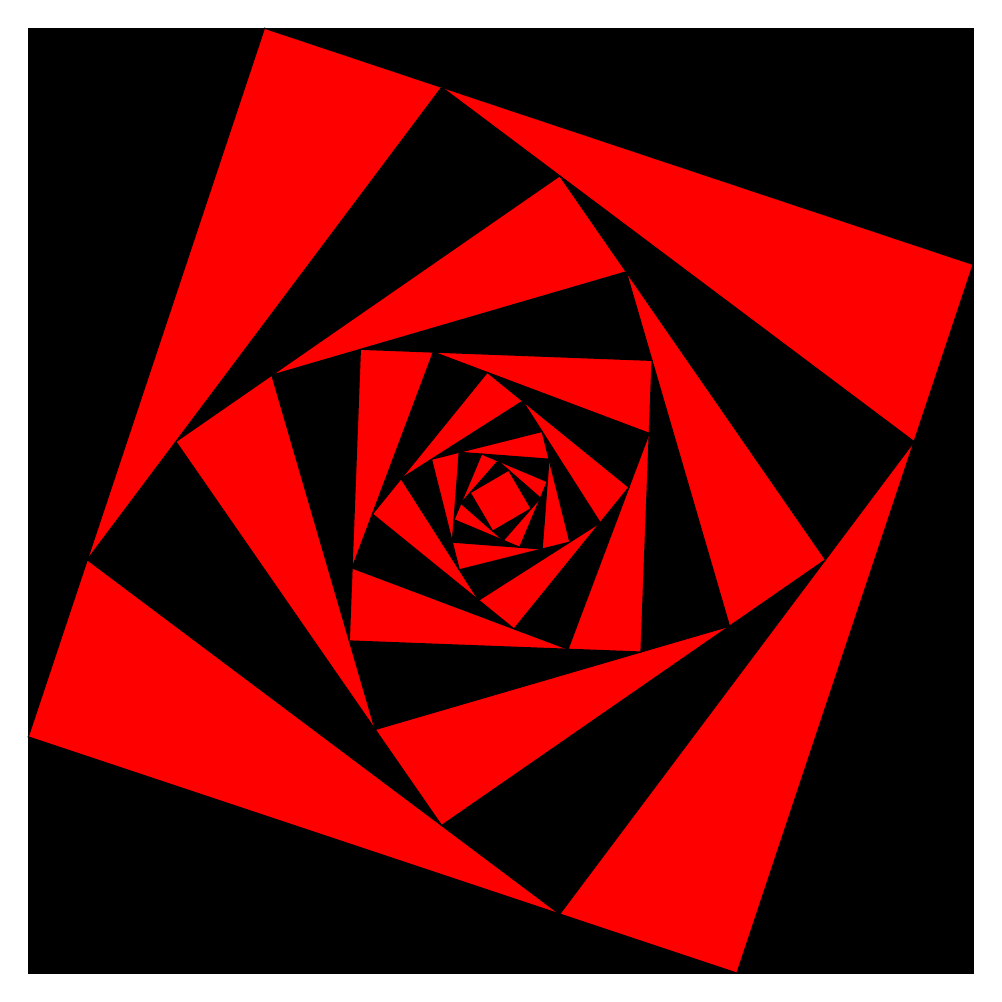
\begin{tikzpicture}
    % Specify the initial square
    \path (0,0) coordinate (A) (12,0) coordinate (B)
          (12,12) coordinate (C) (0,12) coordinate (D);
    \foreach \i in {1,...,14}{
        \ifthenelse{\isodd{\i}}{\def\couleur{black}}{\def\couleur{red}}
        \draw[fill=\couleur] (A)--(B)--(C)--(D)--cycle; 
        \path (A) coordinate (TMP);
        \path (A)--(B) coordinate[near end] (A)
                 --(C) coordinate[near end] (B)
                 --(D) coordinate[near end] (C)
                 --(TMP) coordinate[near end] (D);
    }
\end{tikzpicture}


\end{document}
